% !TEX root = ../mat999.tex
\newpage
\section{Functions and Convergence.}
\subsection{Functions.}
\subsubsection{Bounded ($L^{\infty}$) Functions}
\begin{definition}
A piecewise continuous function $f(x)$ defined on an interval
Is bounded (or $\left.L^{\infty}\right)$ on I there is a number $M>0$ such that $|f(x)| \leq M$ for
all $x \in I .$
The $L^{\infty}$ -norm of a function $f(x)$ is defined by
$$
\|f\|_{\infty}=\sup \{|f(x)|: x \in I\}
$$
\end{definition}

\subsubsection{Integrable ($L^{1}$) Functions}
\begin{definition}
A piecewise continuous function $f(x)$ defined on an interval
Is integrable (or of class $L^{1}$ or simply $L^{1}$ ) on I if the integral
$$
\int_{1}|f(x)| d x
$$
is finite.
The $L^{1}$ -norm of a function $f(x)$ is defined by
$$
\|f\|_{1}=\int_{I}|f(x)| d x
$$
\end{definition}

\subsubsection{Square Integrable ($L^{2}$) Functions}
\begin{definition}
A piecewise continuous function $f(x)$ defined on an interval
I is square-integrable (or of class $L^{2}$ or simply $L^{2}$ ) on I if the integral
$$
\int_{I}|f(x)|^{2} d x
$$
is finite.
The $L^{2}$ -norm of a function $f(x)$ is defined by
$$
\|f\|_{2}=\left(\int_{I}|f(x)|^{2} d x\right)^{1 / 2}
$$
\end{definition}

\subsubsection{Differentiable ($C^{n}$) Functions}
\begin{definition}
Given $n \in \mathbf{N},$ we say that a function $f(x)$ defined on an
interval $I$ is $C^{n}$ on $I$ if it is n-times continuously differentiable on $I . C^{0}$ on I
means that $f(x)$ is continuous on $I . f(x)$ is $C^{\infty}$ on I if it is $C^{n}$ on I for every
$n \in \mathbb{N} .$
We say that $f(x)$ is $C_{c}^{n}$ on I if it is $C^{n}$ on I and compactly supported, $C_{c}^{0}$ on
I if it is $C^{0}$ on I and compactly supported, and $C_{c}^{\infty}$ on I is $C^{\infty}$ on $I$ and
compactly supported.
\end{definition}

\subsection{Convergence of Sequences of Functions}
\subsubsection{Numerical Convergence}
\begin{definition}
 The sequence $\left\{a_{n}\right\}_{n \in \mathbf{N}}$ converges to the number a if for
every $\epsilon>0,$ there is an $N>0$ such that if $n \geq N,$ then $\left|a_{n}-a\right|<\epsilon .$ In this case,
we write $a_{n} \rightarrow a$ as $n \rightarrow \infty,$ or $\lim _{n \rightarrow \infty} a_{n}=a$.
A numerical series, denoted $\sum_{n=1}^{\infty} a_{n},$ converges to a number $S$ if the sequence
of partial sums $\left\{s_{N}\right\}_{N \in \mathrm{N}}$ defined by $s_{N}=\sum_{n=1}^{N} a_{n}$ converges to $S .$ In this
case, we write $\sum_{n=1}^{\infty} a_{n}=S .$ We will frequently denote the series $\sum_{n=1}^{\infty} a_{n}$ by
$\sum_{n \in \mathbf{N}} a_{n} .$

A series $\sum_{n \in \mathrm{N}} a_{n}$ converges absolutely if $\sum_{n \in \mathbf{N}}\left|a_{n}\right|$ converges.

\end{definition}

\begin{ex}
Consider the series $\sum_{n=0}^{\infty} r^{n} .$ The partial sum sequence can be computed since
$$
s_{N}=\sum_{n=0}^{N} r^{n}=\frac{1-r^{N+1}}{1-r}
$$
If $|r|<1,$ then $s_{N} \rightarrow 1 /(1-r)$ as $N \rightarrow \infty .$ Therefore, if $|r|<1,$ then
$$
\sum_{n=0}^{\infty} r^{n}=\frac{1}{1-r}
$$
\end{ex}

\subsubsection{Pointwise Convergence}
\begin{definition}
 A sequence of functions $\left\{f_{n}(x)\right\}_{n \in \mathrm{N}}$ defined on an interval I converges pointwise to a function $f(x)$ if for each $x_{0} \in I,$ the numerical sequence
$\left\{f_{n}\left(x_{0}\right)\right\}_{n \in \mathrm{N}}$ converges to $f\left(x_{0}\right) .$ We write $f_{n}(x) \rightarrow f(x)$ pointwise on $I,$ as
$n \rightarrow \infty$.
The series $\sum_{n=1}^{\infty} f_{n}(x)=f(x)$ pointwise on an interval I if for each $x_{0} \in I,$
$\sum_{n=1}^{\infty} f_{n}\left(x_{0}\right)=f\left(x_{0}\right)$
\end{definition}

\subsubsection{Uniform $(L^{\infty})$ Convergence}
\begin{definition}
 
The sequence \{ $\left.f_{n}(x)\right\}_{n \in \mathbf{N}}$ converges uniformly on I to the
function $f(x)$ if for every $\epsilon>0$, there is an $N>0$ such that if $n \geq N$, then
$\left|f_{n}(x)-f(x)\right|<\epsilon$ for all $x \in I .$ We write $f_{n}(x) \rightarrow f(x)$ uniformly on I as
$n \rightarrow \infty$.
The series $\sum_{n=1}^{\infty} f_{n}(x)=f(x)$ uniformly on I if the sequence of partial sums
$s_{N}(x)=\sum_{n=1}^{N} f_{n}(x)$ converges uniformly to $f(x)$ on $I .$
\end{definition}


\section{Fourier Series}

\subsection{Periodic Functions}

\begin{definition}
Definition 2.1. A function $f(x)$ defined on $\mathbf{R}$ has period $p>0$ if $f(x+p)=$
$f(x)$ for all $x \in \mathbf{R} .$ Such a function is said to be periodic.
\end{definition}

\subsubsection{Periodization}
\begin{definition}
Given a function $f(x)$ on $\mathbf{R} .$ and a number $p>0 .$ the $p$ -
periodization of $f(x)$ is defined as the function
$$
f_{p}(x)=\sum_{n \in \mathbf{Z}} f(x+n p)
$$
provided that the sum makes sense.

\end{definition}

\subsubsection{The Trigonometric System}
\begin{definition}
Given a $>0,$ the collection of functions
$$
\left\{e^{2 \pi i n \tau / a}\right\}_{n \in \mathbf{Z}}
$$
is called the (period a) trigonometric system.
\end{definition}

\subsection{The Fourier Coefficients.}
\begin{definition}
Given a function $f(x)$ with period a, the Fourier coefficients
of $f(x)$ are defined by
$$
c(n)=\frac{1}{a} \int_{0}^{a} f(x) e^{-2 \pi \ln x / a} d x \quad \text { for } \quad n \in \mathbf{Z} .
$$
provided that those integrals make sense. For example. if $f(x)$ is $L^{1}$ on $[0 . a],$ then
the integral converges for each $n$.
\end{definition}

\subsubsection{Fourier Series}
\begin{definition}
Definition 2.11. Given a function $f(x)$ with period a, $L^{1}$ on $[0, a],$ the Fourier
series associated with $f(x)$ is defined as the formal series
$$
\sum_{n \in \mathbb{Z}} c(n) e^{2 \pi i n x / a}
$$
where the $c(n)$ are defined by $(2.4)$ We refer to $(2.5)$ as a "formal series" since
where the $c(n)$ how or if the series converges. We write
$$
f(x) \sim \sum_{n \in \mathbf{Z}} c(n) e^{2 \pi i n x / a}
$$
\end{definition}

\subsubsection{Convergence of Fourier Series.}

\begin{definition}
A function $f(x)$ on a finite interval I is piecewise differentiable on If (a) $f(x)$ is piecewise continuous on I with only jump discontinuities (if any), (b) $f^{\prime}(x)$ exists at all but finitely many points in $I$ and (c) $f^{\prime}(x)$ is piecewise continuous on I with only jump discontinuities (if any). A function $f(x)$ is piecewise differentiable on an infinite interval I if it is piecewise differentiable on every finite subinterval of $I$.
\end{definition}

\begin{theorem}
(Dirichlet) Suppose that $f(x)$ has period a $>0$ and is piecewise differentiable on $\mathbf{R} .$ Then the sequence of partial sums of the Fourier series of $f(x),\left\{S_{N}(x)\right\}_{N \in \mathbf{N}},$ where
$$
S_{N}(x)=\sum_{n=-N}^{N} c(n) e^{2 \pi i n x / a}, \quad c(n)=\frac{1}{a} \int_{0}^{a} f(t) e^{-2 \pi i n x / a} d x,
$$
converges pointwise to the function $\tilde{f}(x),$ where
$$
\tilde{f}(x)=\frac{1}{2}\left[\lim _{t \rightarrow x^{+}} f(t)+\lim _{t \rightarrow x^{-}} f(t)\right]
$$
\end{theorem}

\begin{theorem}
(DuBois-Reymond) There exists a function $f(x)$ continuous on $\mathbf{R}$ and with period $2 \pi$ such that the Fourier series of $f(x)$ diverges at $x=0$.
That is, lim $_{N \rightarrow \infty} S_{N}(0)$ does not exist where $S_{N}(x)$ is given by:
$$
S_{N}(x)=\sum_{n=-N}^{N} c(n) e^{2 \pi i n x / a}, \quad c(n)=\frac{1}{a} \int_{0}^{a} f(t) e^{-2 \pi i n x / a} d x,
$$
\end{theorem}

\begin{figure}[ht]
    \centering
    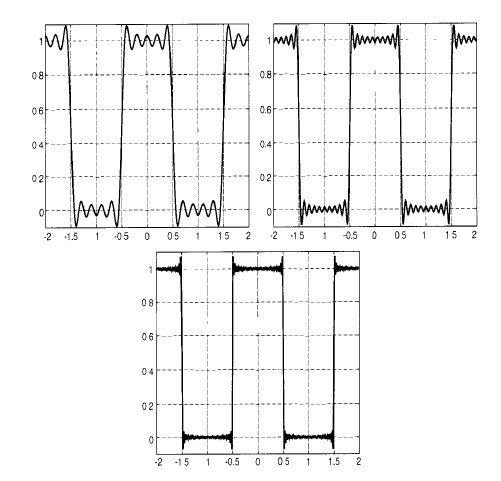
\includegraphics[width=0.4\textwidth]{sections/Gibbs.PNG}
    \caption{Partial sums $S_{N}(x)$ of the Fourier series $f(x)$ (Square Wave) Top left: $N=10,$ top right: $N=20,$ bottom: $N=60 .$}
    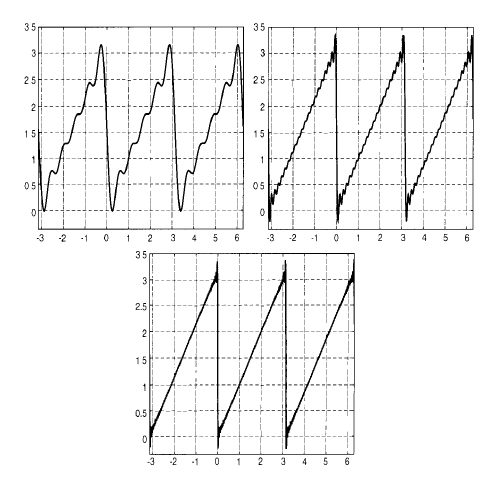
\includegraphics[width=0.4\textwidth]{sections/Gibbs0.PNG}
    \caption{Partial sums $S_{N}(x)$ of the Fourier series $f(x)$ (Saw-tooth wave) .Top left: $N=10,$ top right: $N=20,$ bottom: $N=60 .$}
    \label{fig:Gibbs}
\end{figure}


\begin{theorem}
Theorem 2.19. (Fejer's Theoren) Let $f(x)$ be a function with period a $>0$
continuous on R. and define for each $n \in \mathbf{N}$ the function $\sigma_{N}(x)$ by
$$
\sigma_{N}(x)=\frac{1}{N} \sum_{k=0}^{N-1} S_{k}(x)
$$
where $S_{k }(x)$ is given by (2.1) then,  $ \sigma_{N}(x) $ converges uniformly to $f(x)$ on $\mathbf{R}$ as $N \rightarrow \infty$.
\end{theorem}



\subsection{Orthogonality and Orthonormality.}
\begin{definition}
A collection of functions $\left\{g_{n}(x)\right\}_{n \in \mathrm{N}}, L^{2}$ on an interval $I$ is a (general) orthogonal system on I provided that,


(a) $\int_{I} g_{n}(x) \overline{g_{m}(x)} d x=0$ if $n \neq m,$ and,


(b) $\int_{I} g_{n}(x) \overline{g_{n}(x)} d x=\int_{I}\left|g_{n}(x)\right|^{2} d x>0$


Part (b) says in particular that none of the $g_{n}(x)$ can be identically zero.
The collection $\left\{g_{n}(x)\right\}_{n \in \mathbb{N}}$ is a (general) orthonormal system on I provided that it is an orthogonal system on I, and 

(b') $\int_{I} g_{n}(x) \overline{g_{n}(x)} d x=\int_{I}\left|g_{n}(x)\right|^{2} d x=1$.
\end{definition}

\subsection{Generalized Fourier Series.}

\begin{definition}
Given a function $f(x), L^{2}$ on an interval $I,$ and an orthonormal system $\left\{g_{n}(x)\right\}$ on $I,$ the (generalized) Fourier coefficients, $\{c(n)\}$ of $f(x)$ with respect to $\left\{g_{n}(x)\right\}$ are defined by
$\qquad\{ c(n)\}$ are defined by
$$
c(n)=\int_{I} f(x) \overline{g(x)} d x=\left\langle f, g_{n}\right\rangle
$$
The (generalized) Fourier series of $f(x)$ with respect to $\left\{g_{n}(x)\right\}$ is
$$
f(x) \sim \sum_{n \in \mathbb{N}}\left\langle f, g_{n}\right\rangle g_{n}(x)
$$
$$
n \in \mathbb{N}
$$
\end{definition}

\section{The Fourier Transform}
\begin{definition}
 The Fourier transform of a function $f(x) . L^{1}$ on $\mathbf{R} .$ is also a function on $\mathbf{R} .$ denoted $\widehat{f}(\gamma)$ defined by
$$
\widehat{f}(\gamma)=\int_{\mathbf{R}} f(x) e^{-2 \pi i \gamma x} d x
$$
\end{definition}

The assumption that $f(x)$ is $L^{1}$ on $\mathbf{R}$ is made in order to ensure that the integral in ( 3.4) converges for each number $\gamma$. This convergence holds by virtue of the fact that for each $\gamma \in \mathbf{R},$ we can establish a Cauchy condition on the numbers

$$
s_{a}^{+}=\int_{0}^{a} f(x) e^{-2 \pi i \gamma x} d x \quad and \quad s_{a}^{-}=\int_{-a}^{0} f(x) e^{-2 \pi i \gamma x} d x, \quad a>0
$$

\subsection{Fourier Inversion}

\begin{theorem}
If $f(x)$ is $C^{0}$ and $L^{1}$ on $\mathbf{R},$ then for each $x \in \mathbf{R}$,
$$
\lim _{\tau \rightarrow 0^{+}} \int_{\mathbf{R}} \widehat{f}(\gamma) e^{-\pi \tau^{2} \gamma^{2}} e^{2 \pi \imath \gamma x} d \gamma=f(x)
$$

\begin{corollary}
If $f(x)$ is $C^{0}$ and $L^{1}$ on $\mathbf{R},$ and if $\hat{f}(\gamma)$ is $L^{1}$ on $\mathbf{R},$ then
for each $x \in \mathbf{R}$,
$$
\int_{\mathbf{R}} \widehat{f}(\gamma) e^{2 \pi i \gamma x} d \gamma=f(x)
$$
\end{corollary}
\end{theorem}

\subsection{Plancherel's Formula}

If $f(x)$ is $L^{1}$ and $L^{2}$ on $\mathbf{R},$ then 
$\hat{f}(\gamma)$
is also $L^{2}$ on $\mathbf{R}$ and
$$
\int_{\mathbf{R}}|\widehat{f}(\gamma)|^{2} d \gamma=\int_{\mathbf{R}}|f(x)|^{2} d x
$$

\begin{theorem}
(General) If $f(x)$ and $g(x)$ are both $L^{1}$ and $L^{2}$ on
$\mathbf{R},$ then
$$
\int_{\mathbf{R}} \widehat{f}(\gamma) \overline{\widehat{g}(\gamma)} d \gamma=\int_{\mathbf{R}} f(x) \overline{g(x)} d x
$$
\end{theorem}

\subsection{The Discrete Fourier Transform}
\subsubsection{DFT}
\begin{definition}
Given a period $N$ signal $x(n),$ the $(N-\text { point })$ Discrete Fourier Transform or $(N-\text { point) DFT of } x(n), \text { denoted } \widehat{x}(n), \text { is the period } N$ sequence defined by:
$$
\widehat{x}(n)=\sum_{j=0}^{N-1} x(j) e^{-2 \pi i y n / N}
$$
\end{definition}

\subsubsection{IDFT}
\begin{definition}
Given a period $N$ sequence $x(n)$ with $D F T \widehat{x}(n)$
$$
x(j)=\frac{1}{N} \sum_{n=0}^{N-1} \widehat{x}(n) e^{2 \pi i n j / N}
$$
for each $j \in \mathbf{Z}$.
\end{definition}


\section{Dilation, Translation, and Modulation}

\begin{definition}
 Given a>0, the dilation operator, Da, defined on functions
$f(x), L^{1}$ or $L^{2}$ on $\mathbf{R},$ is given by
$$
D_{a} f(x)=a^{1 / 2} f(a x)
$$
Given $b \in \mathbf{R},$ the translation operator, $T_{b},$ defined on functions $f(x), L^{1}$ or $L^{2}$
on $\mathbf{R},$ is given by
$$
T_{b} f(x)=f(x-b)
$$
Given $c \in \mathbf{R},$ the modulation operator, $E_{c},$ defined on functions $f(x), L^{1}$ or $L^{2}$
on $\mathbf{R},$ is given by
$$
E_{c} f(x)=e^{2 \pi t c x} f(x)
$$

\end{definition}

\begin{theorem}

For any function $f(x) L^{1}$ on $\mathbf{R}$,

(a) For every $a>0, \widehat{D_{a} f}(\gamma)=D_{1 / a} \widehat{f}(\gamma)$

(b) For every $b \in \mathbf{R}, \widehat{T_{b} f}(\gamma)=E_{-b} \widehat{f}(\gamma)$

(c) For every $c \in \mathbf{R}, \widehat{E_{r} f}(\gamma)=T_{c} \widehat{f}(\gamma)$
\end{theorem}

\begin{theorem}
(Properties of Dilation and Translation) For every $f(x)$ and
$g(x), L^{2}$ on $\mathbf{R},$ and for every $a>0, b \in \mathbf{R},$ the following hold.

(a) $D_{a} T_{b} f(x)=a^{1 / 2} f(a x-b)$

(b) $D_{a} T_{b} f(x)=T_{a}-1_{b} D_{a} f(x)$

(c) $\left\langle f, D_{a} g\right\rangle=\left\langle T_{-b} f, g\right\rangle$

(d) $\left\langle f, T_{b} g\right\rangle=\left\langle T_{-b} D_{a^{-}}-1, g\right\rangle$

(e) $\left\langle f, D_{a} T_{b} g\right\rangle=\left\langle T_{-b} D_{a^{-}}-1, g\right\rangle$

(f) $\left\langle D_{a} f, D_{a} g\right\rangle=\langle f, g\rangle$

(g) $\left\langle T_{b} f, T_{b} g\right\rangle=\langle f, g\rangle$
\end{theorem}


\section{The Haar System.}

\subsection{The Haar Scaling Functions and the Haar Functions.}

\begin{definition}
Let $p(x)=X_{[0.1)}(x),$ and for each $j . k \in \mathbf{Z},$ define 

$$
p_{j . k}(x)=2^{j / 2} p\left(2^{j}, r-k\right)=D_{2}, T_{k} p(x)
$$

The collection $\left\{p_{j, k}(x)\right\}_{\text {t. } k \in \mathbf{Z}}$ is referred to as the system of Haar scaling function. For each $j \in \mathbf{Z}$. the collection $\left\{p_{1, k}(x)\right\}_{k \in \mathbf{Z}}$ is referred to as the system of
scale $j$ Haar scaling functions.

Let $h(x)=\chi_{[0,1 / 2)}(x)-\chi_{[1 / 2,1]}(x),$ and for each $j, k \in \mathbf{Z}$, define
$$
h_{j, k}(x)=2^{J / 2} h\left(2^{j} x-k\right)=D_{2^{j}} T_{k} h(x)
$$
The collection $\left\{h_{j, k}(x)\right\}_{j, k \in \mathbf{Z}}$ is referred to as the Haar system on $\mathbf{R}.$ For each $j \in \mathbf{Z},$ the collection $\left\{h_{J, k}(x)\right\}_{k \in \mathbf{Z}}$ is referred to as the system of scale $j$ Haar functions.
\end{definition} 


\textbf{Properties:}

\begin{itemize}
    \item For each $j . k \in \mathbf{Z}, p_{j . k}(x)=2^{j / 2} \mathrm{l}_{I_{j . k}}(x) .$ so that $p_{j . k}(x)$ is supported on the interval $I_{j . k}$ and does not vanish on that interval. Therefore, we refer to the scaling function $p_{j . k}(. r)$ as being associated with the interval $I_{j, k} .$
    
    \item For each $j, k \in \mathbf{Z}$
    $$
       \int_{\mathbf{R}} p_{j, k}(x) d x=\int_{I_{j, k}} p_{j, k}(x) d x=2^{-j / 2}
    $$
    and
    $$
       \int_{\mathbf{R}}\left|p_{j, k}(x)\right|^{2} d x=\int_{I_{j, k}}\left|p_{j, k}(x)\right|^{2} d x=1
    $$
\end{itemize}

\subsection{The Haar Bases on [0,1].}

For any integer $J \geq 0,$ the scale $J$ Haar system on $[0,1]$ is
the collection
$$
\left\{p_{J, k}(x): 0 \leq k \leq 2^{J}-1\right\} \cup\left\{h_{J, k}(x): j \geq J ; 0 \leq k \leq 2^{J}-1\right\}
$$
When $J=0,$ this collection will be referred to simply as the Haar system on $[0,1] .$

(a) The Haar system on $[0,1]$ consists of precisely those Haar functions $h_{j, k}(x)$ corresponding to dyadic intervals $I_{j, k}$ that are sub-
sets of $[0,1],$ together with the single scaling function $p_{0,0}(x)$

(b) For $J>0,$ the scale $J$ Haar system on $[0,1]$ consists of precisely those
Haar functions $h_{j, k}(x)$ corresponding to dyadic intervals $I_{j . k}$ for which $j \geq$
$J$ and that are subsets of $[0,1],$ together with those scale $J$ Haar scaling
functions that are supported in $[0,1] .$

\begin{figure}[h]
    \centering
    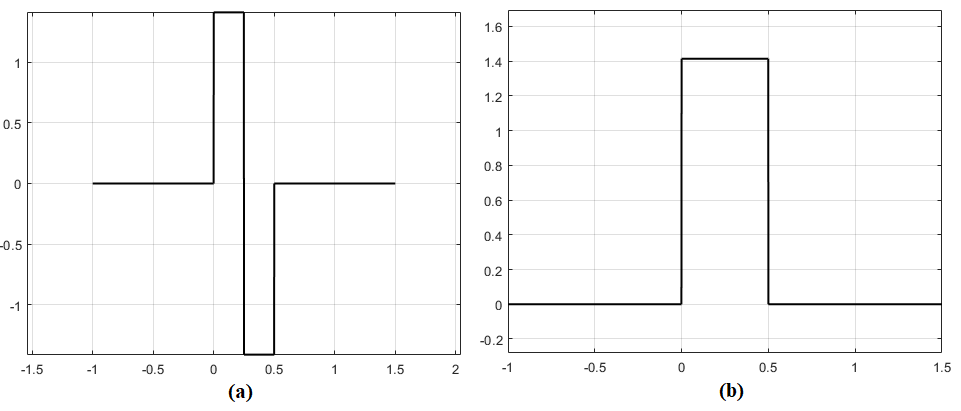
\includegraphics[width=\textwidth]{sections/Haar_Basis.PNG}
    \caption{(a) The Haar functions $h_{\jmath, k}(x)$ on $[0,1)$, (b)Haar scaling function $p_{j, k}(x)$ on $[0,1)$.}
    \label{fig:Haar}
\end{figure}


\subsection{Approximate and Detailed Operators.}


\begin{definition} For each $j \in \mathbf{Z},$ define the approximation operator $P_{j}$ on
functions $f(x), L^{2}$ on $\mathbf{R}, b y$
$$
P_{J} f(x)=\sum_{k}\left\langle f, p_{J, k}\right\rangle p_{\jmath, k}(x)
$$
\end{definition}

(a) For each $j \in \mathbf{Z}$, define the approximation space $V_{j}$ by
$$
V_{j}=\overline{\operatorname{span}}\left\{p_{\jmath, k}(x)\right\}_{k \in \mathbf{Z}}
$$

since $\left\{p_{\jmath, k}(x): k \in \mathbf{Z}\right\}$ is an orthonormal system on $\mathbf{R} \in \mathbf{Z}$.
that $P_{j} f(x)$ is the function in $V_{j}$ best approximating $f(x)$ in the $L^{2}$ sense.

(b) since $p_{j, k}(x)=2^{j / 2} \chi_{I_{j, k}}(x)$
$$
\qquad\left(f, p_{j, k}\right) p_{j, k}(x)=\left(2^{j} \int_{I_{j, k}} f(t) d t\right) \chi_{I_{j, k}}(x) 
$$
In other words, on the interval $ I_{j, k}, P_{j} f(x)$ is the average value of $f(x)$ on ${I_{J, k}}$


\begin{definition}
For each $j \in \mathbf{Z},$ define the detail operator $Q_{j}$ on functions
$f(x), L^{2}$ on $\mathbf{R}, b y$
$$
Q_{j} f(x)=P_{j+1} f(x)-P_{j} f(x)
$$
\end{definition} 
\begin{figure}[h]
    \centering
    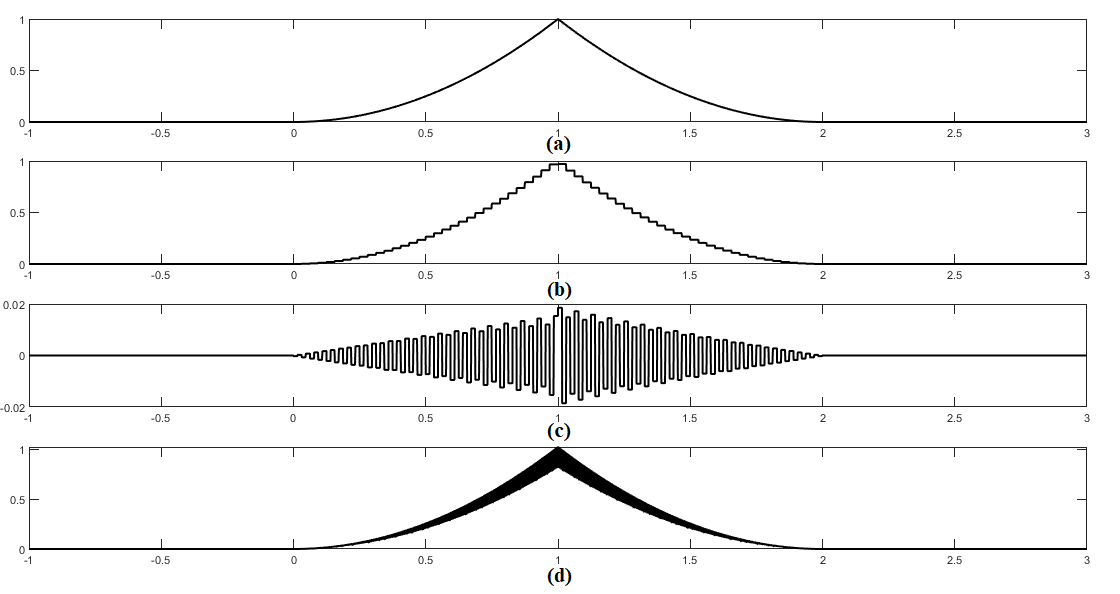
\includegraphics[width=\textwidth]{sections/PxQxFx.png}
    \caption{(a) Approximate Operator of Hat function, (b) Approximate Operator of Second Degree Hat function, (c) Detailed Operator of Second Degree Hat function, (d)Approximation of Second Degree Hat function Using Haar Basis.}
    \label{fig:PxQxFx}
\end{figure}


(a) For each $j \in \mathbf{Z},$ we define the wavelet space $W_{j}$ by
$$
W_{j}=\overline{\operatorname{span}}\left\{h_{J, k}(x)\right\}_{k \in \mathbf{Z}}
$$
since $\left\{h_{j, k}(x)\right\}_{k \in \mathbf{Z}}$ is an orthonormal system on $\mathbf{R}$ implies that $Q_{j} f(x)$ is the function in $W_{j}$ best approximating $f(x)$ in the $L^{2}$ sense.

(b) In light of the interpretation of $P_{j} f(x)$ as the blurred version of $f(x)$ at scale $2^{-j},$ we can interpret $Q_{j} f(x)$ as containing those features of $f(x)$ that are of size smaller than $2^{-J}$ but larger than $2^{-\jmath-1} .$ That is, $Q_{j} f(x)$ has those details invisible to the approximation $P_{j} f(x)$ but visible to the approximation $P_{J+1} f(x)$

\section{The Discrete Haar Transform in 1 Dimension.}

\subsection{Motivation.}
A function $f(x)$ (defined on [ 0.1] his an expansion in terms of
Haar functions as follows. Give that any integer $J \geq 0$.
$$
f(x)=\sum_{j=J}^{x} \sum_{k=0}^{2^{\prime}-1}\left\langle f \cdot h_{j \cdot k}\right\rangle h_{J, k} \cdot(x)+\sum_{k=0}^{2^{\prime}-1}\left\langle f \cdot p_{J, k}\right\rangle p_{J, k}(x)
$$

in $L^{2}$ on $[0.1]$

Thus. the Haar coefficients of $f(x)$ can be approximated by the Haar coefficients of $P_{N} f(x)$. That is.
$$
\left\langle f . h_{J,k}\right\rangle \approx\left\langle P_{N} f . h_{J,k}\right\rangle \quad \text { and } \quad\left\langle f, p_{J,k}\right\rangle \approx\left\langle P_{N} f, p_{J,k}\right\rangle
$$

\subsection{DHT \& IDHT}

\begin{definition}
Suppose that we are given a finite sequence of data of length $2^{N}$ for some
$N \in \mathbf{N} .\left\{c_{0}(k)\right\}_{k=0}^{2}-1$. We assume that for some underlying function $f(x)$
$c_{0}(k)=\left\langle f \cdot p_{N, k}\right\rangle .$ Fix $J \in \mathbf{N} . J<N .$ and for each $1 \leq j \leq J,$ define,

$c_{j}(k)=\left\langle f, p_{N-j, k}\right\rangle \quad$ and $\quad d_{j}(k)=\left\langle f . h_{N-j . .\rangle}\right\rangle$

\end{definition}

It turns out that there is a convenient recursive algorithm that can be used to compute the coefficients $c_{j}(k)$ and $d_{j}(k)$ from $c_{j-1}(k) .$.

$\begin{aligned} c_{j}(k) &=\left\langle f, p_{N}-, . k\right\rangle \\ &=\frac{1}{\sqrt{2}}\left\langle f, p_{N}-j+1.2 k\right\rangle+\frac{1}{\sqrt{2}}\left\langle f \cdot p_{N}-j+1,2 k+1\right\rangle \\ &=\frac{1}{\sqrt{2}} c_{J-1}(2 k)+\frac{1}{\sqrt{2}} c_{J-1}(2 k+1) \\ &=\frac{1}{\sqrt{2}} c_{j-1}(2 k)-\frac{1}{\sqrt{2}} c_{j-1}(2 k+1) \end{aligned}$

$d_{j}(k)=\frac{1}{\sqrt{2}} c_{j-1}(2 k)-\frac{1}{\sqrt{2}} c_{j-1}(2 k+1)$

By writing in Matrix form,
$$
\left(\begin{array}{c}{c_{j}(k)} \\ {d_{j}(k)}\end{array}\right)=\frac{1}{\sqrt{2}}\left(\begin{array}{cc}{1} & {1} \\ {1} & {-1}\end{array}\right)\left(\begin{array}{c}{c_{j-1}\left(2 k_{i}\right)} \\ {c_{j-1}(2 k+1)}\end{array}\right)
$$

$$
\left(\begin{array}{c}{c_{j-1}(2 k)} \\ {\left( c_{j-1}(2 k+1)\right.}\end{array}\right)=\frac{1}{\sqrt{2}}\left(\begin{array}{cc}{1} & {1} \\ {1} & {-1}\end{array}\right)\left(\begin{array}{c}{c_{j}(k)} \\ {d_{j}(k)}\end{array}\right)
$$

As with the DFT, the DHT can be thought of as a linear transformation on a finite-dimensional space and as such can be written as multiplication by a matrix.

\begin{definition}

Given $L \in \mathbf{N}$ even, define the $(L / 2) \times L$ matrices $H_{L}$ and $G_{L}$ by:

$$
H_{L}=\frac{1}{\sqrt{2}}\left(\begin{array}{cccccc}{1} & {1} & {0} & {} & {\cdots} & {0} \\ {0} & {0} & {1} & {1} & {0} & {\cdots} & {0} \\ {} & {} & {} & {\vdots} & {} \\ {0} & {} & {\cdots} & {} & {0} & {1} & {1}\end{array}\right)
$$

$$
G_{L}=\frac{1}{\sqrt{2}}\left(\begin{array}{cccccc}{1} & {-1} & {0} & {} & {\cdots} & {0} \\ {0} & {0} & {1} & {-1} & {0} & {\cdots} & {0} \\ {} & {} & {} & {\vdots} \\ {0} & {} & {\cdots} & {} & {0} & {1} & {-1}\end{array}\right)
$$

Define the $L \times L$ matrix $\mathcal{W}_{L}$ by
$$
\mathcal{W}_{L}=\left(\begin{array}{c}{H_{L}} \\ {G_{L}}\end{array}\right)
$$
The matrix $H_{L}$ is referred to as the approximation matrix, the matrix $G_{L}$ as the detail matrix, and the matrix $\mathcal{W}_{L}$ as the wavelet matrix.
\end{definition}

\subsubsection{Algorithms for DHT and IDHT}

\begin{definition}
Given $J, N \in \mathbf{N}$ with $J<N$ and a vector
$$
\mathbf{c}_{0}=\left(c_{0}(0) c_{0}(1) \cdots c_{0}\left(2^{N}-1\right)\right)
$$
of length $2^{N},$ the $D H T$ of $\mathbf{c}_{0}$ is the vector
$$
\left(\begin{array}{ll}{d_{1}} & {d_{2}}\end{array} \cdots d_{J} c_{J}\right)
$$
where,
$$
\left(\begin{array}{c}{\mathbf{c}_{J}} \\ {\mathbf{d}_{j}}\end{array}\right)=\left(\begin{array}{c}{H} \\ {G}\end{array}\right) \mathbf{c}_{\jmath-1}
$$
\end{definition} 
\begin{figure}[h]
    \centering
    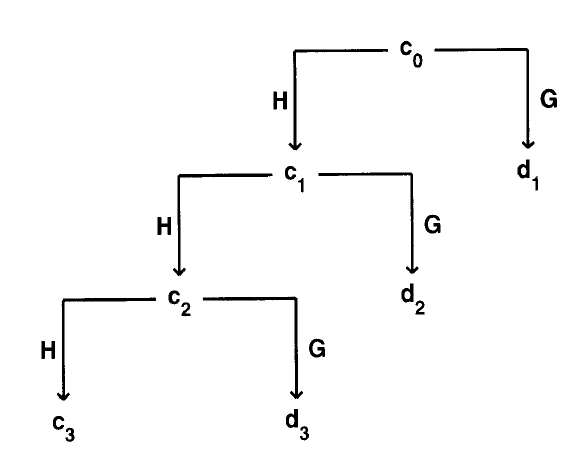
\includegraphics[width=0.5\textwidth]{sections/Tree.PNG}
    \caption{Tree Diagram for The DHT.}
    \label{fig:DHTS}
\end{figure}


\section{The Discrete Haar Transform in 2 Dimensions.}

In many applications, especially image processing, the objects being analyzed are best thought of as matrices, rather than one-dimensional finite signals. That is, we are interested in $L \times M$ matrices $c$ of the form $c=\{c(n, m): 0 \leq n \leq L-1 ; 0 \leq m \leq M-1\} .$ The purpose of this section is to define a generalization of the DHT for matrices.

Given an even number $L \in \mathbf{N},$ let $H$ and $G$ be the $(L / 2) \times L$ matrices. Let $c$ be an $M \times L$ matrix of the form
$$
c=\left(\begin{array}{c}{c_{0}} \\ {c_{1}} \\ {\cdots} \\ {c_{M-1}}\end{array}\right)
$$

In this notation, $c_{\ell}$ is the $\ell$ th row of $c .$ We define the row-wise approximation matrix of $c, \mathbf{H}^{\text {row }} c,$ to be the $M \times(L / 2)$ matrix defined by
$$
\mathbf{H}^{\text {row }} c=\left(\begin{array}{c}{H c_{0}} \\ {\text { He}_{1}} \\ {\cdots} \\ {H c_{M-1}}\end{array}\right)
$$

We define the row-wise detail matrix of $c,$ Grow $c, |$ to be the $M \times(L / 2)$
matrix defined by:
$$
\mathbf{G}^{\text {row }} c=\left(\begin{array}{c}{G c_{0}} \\ {G c_{1}} \\ {\cdots} \\ {G c_{M-1}}\end{array}\right)
$$


Given $L \in \mathbf{N}$ even, let $c$ be an $L \times M$ matrix of the form
$$
c=\left(\begin{array}{cccc}{c_{0}} & {c_{1}} & {\cdots} & {c_{M-1}}\end{array}\right)
$$
where $c_{\ell}$ is the $\ell^{t h}$ column of $c$. We define the column-wise approximation matrix of $c, \mathbf{H}^{\operatorname{col}} c,$ to be the $(L / 2) \times M$ matrix defined by
$$
\mathbf{H}^{\operatorname{col}} c=\left(\begin{array}{cccc}{H c_{0}} & {H c_{1}} & {\cdots} & {H c_{M-1}}\end{array}\right)
$$

We define the column-wise detail matrix of $c, \mathrm{G}^{\mathrm{rOW}} c,$ to be the $(L / 2) \times M$ matrix defined by
$$
\mathrm{G}^{\mathrm{col}} c=\left(\begin{array}{cccc}{G c_{0}} & {G c_{1}} & {\cdots} & {G c_{M-1}}\end{array}\right)
$$

\subsection{The DHT for the Matrices.}

Given J, $N \in \mathbf{N}$ with $J<N$ and a matrix $c_{0}=\{c(n, m)\}_{n, m=0}^{N-1}$
For $1 \leq j \leq J,$ define the 2 $^{N-3} \times 2^{N-j}$ matrices $c_{j} d_{j}^{(1)}, d_{j}^{(2)},$ and $d_{j}^{(3)}$ by
$$
\begin{aligned} c_{j} &=\mathbf{H}^{\text {col }} \mathbf{H}^{\text {row }} c_{j-1} \\ d_{j}^{(1)} &=\mathbf{G}^{\text {col }} \mathbf{H}^{\text {row }} c_{j-1} \\ d_{j}^{(2)} &=\mathbf{H}^{\text {col }} \mathbf{G}^{\text {row }} c_{j-1} \\ d_{j}^{(3)} &=\mathbf{G}^{\text {col }} \mathbf{G}^{\text {row }} c_{j-1} \end{aligned}
$$

where $\mathbf{H}^{\mathrm{col}}, \mathbf{G}^{\mathrm{col}}, \mathbf{H}^{\mathrm{row}},$ and $\mathbf{G}^{\mathrm{row}}$ are the $2^{N-j-2} \times 2^{N-j-1}$. The $D H T$ of $c_{0}$ is the collection of matrices
$$
\left\{d_{j}^{(1)}, d_{j}^{(2)}, d_{j}^{(3)}\right\}_{j=1}^{J} \cup\left\{c_{J}\right\}
$$


\subsection{The IDHT for the Matrices.}

Given $L \in \mathbb{N}$, let $H^{*}$ alld $G^{*}$ loc the adjoints of $H$ and $G$. Let $c$ be
all $M \times(L / 2)$ matrix of the form,
$$
c=\left(\begin{array}{c}{c_{1}} \\ {c_{1}} \\ {\cdots} \\ {c_{M-1}}\end{array}\right)
$$
We define the row-wise approximation adjoint of $r . \mathbf{H}^{\mathrm{rOW}^{*}} c$. to be the $M \times L$ Matrix.

$$
\mathbf{H}^{\mathrm{row} *} c=\left(\begin{array}{c}{H^{*} c_{0}} \\ {H^{*} c_{1}} \\ {\cdots} \\ {H^{*}(n /-1)}\end{array}\right)
$$

We define the row-wise detail adjoint of $C . \mathrm{G}^{\mathrm{row} *}$ c. to be the $M \times L$ matrix
$$
\mathrm{G}^{\mathrm{row}^{*}} c=\left(\begin{array}{c}{G^{*} c_{0}} \\ {G^{*} c_{1}} \\ {\cdots} \\ {G^{*} c_{M-1}}\end{array}\right)
$$

${H_{row}}^{c}$ is the matrix obtained by multiplying each row of $c$ by the matrix
$H^{*},$ and $\mathrm{G}^{\mathrm{row}^{*}} c$ is the matrix obtained by multiplying each row of $c$ by the matrix $G^{*}$. Given $L \in \mathbb{N}$ even, let $c$ be an $(L / 2) \times M$ matrix of the form
$$
c=\left(\begin{array}{cccc}{c_{0}} & {c_{1}} & {\cdots} & {c_{M-1}}\end{array}\right)
$$
We define the column wise approximation adjoint of $c . \mathbf{H}^{\mathrm{col}^{*}} c .$ to be this $L \times M$ matrix,

$$
\mathbf{H}^{\mathrm{COl}^{*}} c=\left(\begin{array}{cccc}{H^{*} c_{0}} & {H^{*} c_{1}} & {\cdots} & {H^{*} c_{M-1}}\end{array}\right)
$$
We define the column-wise detail adjoint of $c .$ Grow $_{C} .$ to be the $L \times M$
matrix
$$
\mathbf{G}^{\mathrm{col}^{*}} c=\left(\begin{array}{cccc}{G^{*} c_{0}} & {G^{*} c_{1}} & {\cdots} & {G^{*} c_{M-1}^{*}}\end{array}\right)
$$

The inverse $D H T$ for matrices is given by
$$
\begin{aligned} c_{3-1}=\mathbf{H}^{\mathrm{row}^{*}} \mathbf{H}^{\mathrm{col}^{*}} c_{3}+\mathbf{H}^{\mathrm{row}^{*}} \mathbf{G}^{\mathrm{col}^{*}} d_{j}^{(1)} \\ &+\mathbf{G}^{\mathrm{row}^{*}} \mathbf{H}^{\mathrm{col}^{*}} d_{3}^{(2)}+\mathbf{G}^{\mathrm{row}^{*}} \mathbf{G}^{\mathrm{col}^{*}} d_{j}^{(3)} \end{aligned}
$$
where $\mathbf{H}^{\mathrm{col}}, \mathbf{G}^{\mathrm{col}}, \mathbf{H}^{\mathrm{row}},$ and $\mathbf{G}^{\mathrm{row}}$ are $2^{N-3-2} \times 2^{N-3-1}$ matrices given above.


\section{Multiresolution Analysis}

\subsection{Orthonormal System of Translates}
\begin{definition}
An orthonormal system on $\mathbf{R}$ of the form $\left\{T_{n} g(x)\right\}_{n \in \mathbf{Z}}$ where $g(x)$ is $L^{2}$ on $\mathbf{R}$ is called an orthonormal system of translates.
\end{definition}

The collection $\left\{T_{n} g(x)\right\}$ is an orthonormal system of translates
if and only if for all $\gamma \in \mathbf{R}$,
$$
\sum_{n}|\widehat{g}(\gamma+n)|^{2} \equiv 1
$$


\subsection{Definition of Multiresolution Analysis}

\begin{definition}
Definition $7.12 .$ A multiresolution analysis on $\mathbf{R}$ is a sequence of subspaces
$\left\{V_{y}\right\}_{y \in \mathbf{Z}}$ of functions $L^{2}$ on $\mathbf{R}$ satisfying the following properties.
\begin{enumerate}
    
\item  For all $j \in \mathbf{Z}, V_{J} \subseteq V_{\jmath+1}$

\item  If $f(x)$ is $C_{c}^{0}$ on $\mathbf{R},$ then $f(x) \in \operatorname{span}\left\{V_{y}\right\}_{g \in \mathbf{Z}} .$ That is, given $\epsilon>0,$ there
$\quad$ is $a j \in \mathbf{Z}$ and a function $g(x) \in V_{\jmath}$ such that $\|f-g\|_{2}<\epsilon$

\item  $\cap_{\jmath \in \mathbf{Z}} V_{\jmath}=\{0\}$

\item  $A$ function $f(x) \in V_{0}$ if and only if $D_{2^{\prime}} f(x) \in V_{j}$.

\item  There exists a function $\varphi(x), L^{2}$ on $\mathbf{R},$ called the scaling function such that the collection $\left\{T_{n} \varphi(x)\right\}$ is an orthonormal system of translates and
$$
V_{0}=\frac{ }{\operatorname{span}}\left\{T_{n} \varphi(x)\right\}
$$
\end{enumerate}
\end{definition}


\subsection{Basic Properties of MRA}
\subsubsection{The Approximation and Detail Operators}
\begin{definition}

For each $j, k \in \mathbf{Z}$ define $\varphi_{j, k}(x)$  by
$$
\varphi_{j, k}(x)=2^{y / 2} \varphi\left(2^{j} x-k\right)=D_{2} s T_{k} \varphi(x)
$$
For each $j \in \mathbf{Z},$ define the approximation operator $P_{j}$ on functions $f(x), L^{2}$ on$\mathbf{R}$ by

$$
P_{J} f(x)=\sum_{k}\left\langle f, \varphi_{j, k}\right\rangle \varphi_{\jmath, k}(x)
$$

For each $j \in \mathbf{Z},$ define the detail operator $Q_{3}$ on functions $f(x), L^{2}$ on $\mathbf{R} b y$
$Q_{j} f(x)=P_{j+1} f(x)-P_{j} f(x)$
\end{definition}

For all $f(x), C_{c}^{0}$ on $\mathbf{R}:$

(a) $\lim _{\vartheta \rightarrow \infty}\left\|P_{\jmath} f-f\right\|_{2}=0,$ and

(b) $\lim _{j \rightarrow-\infty}\left\|P_{\jmath} f\right\|_{2}=0$

There exists an $\ell^{2}$ sequence of coefficients $\{h(k)\}$ such that
$$
\varphi(x)=\sum_{k} h(k) 2^{1 / 2} \varphi(2 x-k)
$$
in $L^{2}$ on R. Moreover, we may write
$$
\hat{\varphi}(\gamma)=m_{0}(\gamma / 2) \widehat{\varphi}(\gamma / 2)
$$
where
$$
m_{0}(\gamma)=\frac{1}{\sqrt{2}} \sum_{k} h(k) e^{-2 \pi i k \gamma}
$$

\begin{definition}

Let $\varphi(x)$ be the scaling function associated with an MRA $\left\{V_{j}\right\} .$ The sequence $\{h(k)\}$ satisfying (8.2) is called the scaling filter associated
with $\varphi(x) .$ The function $m_{0}(\gamma)$ is called the auxiliary function associated with $\varphi(x) .$
\end{definition}


\section{The Discrete Wavelet Transform}

\subsection{The Approximation and Detail Operators and Their
Adjoints}

\begin{definition}

Let $c(n)$ be a signal.
(a) Given $m \in \mathbf{Z},$ the shift operator $\tau_{m}$ is defined by
$$
\tau_{m} c(n)=c(n-m)
$$

(b) The downsampling operator $\downarrow$ is defined by
$$
(\downarrow c)(n)=c(2 n)
$$
$\text { (Note: ( }t c)(n) \text { is formed by removing every odd term in } c(n) .)$

(c) The upsampling operator $\uparrow$ is defined by
$$
(\uparrow c)(n)=\left\{\begin{array}{cc}{c(n / 2)} & {\text { if } n \text { is even }} \\ {0} & {\text { if } n \text { is odd. }}\end{array}\right.
$$

\end{definition}

\begin{definition}
Given a signal $c(n)$ and a filter h(k), define g(k) by (7.23).
Then the approximation operator $H$ and detail operator $G$ corresponding to $h(k)$ are defined by
$g(k)=(-1)^{k} \overline{h(1-k)}$

$$
(H c)(k)=\sum_{n} c(n) \overline{h(n-2 k)}, \quad(G c)(k)=\sum_{n} c(n) \overline{g(n-2 k)}
$$
\end{definition}

(a) The operators $H$ and $G$ can be thought of as con-
volution with the filters $h(n)=h(-n)$ and $\underline{g}(n)=g(-n)$ followed by
downsampling. That is,
$$
(H c)(n)=\downarrow(c * \underline{h})(n) \quad \text { and } \quad(G c)(n)=\downarrow(c * g)(n)
$$

(b) $H^{*}$ and $G^{*}$ can be thought of as upsampling followed by convolution
with $h$ and $g(x)$. That is,
$$
\left(H^{*} c\right)(n)=(\uparrow c) * h(n) \quad \text { and } \quad\left(G^{*} c\right)(n)=(\uparrow c) * g(n)
$$

(c) The operators $H^{*}$ and $G^{*}$ are the formal adjoints of $H$ and $G .$ That is, for all signals $c(n)$ and $d(n)$,
$$
\langle H c, d\rangle=\sum_{k}(H c)(k) \overline{d(k)}=\sum_{k} c(k) \overline{\left(H^{*} d\right)(k)}=\left\langle c . H^{*} d\right\rangle
$$
$$
\langle H c, d\rangle=\sum_{k}(H c)(k) \overline{d(k)}=\sum_{k} c(k) \overline{\left(H^{*} d\right)(k)}=\left\langle c . H^{*} d\right\rangle
$$

(d)
$$
 {\qquad\langle G c, d\rangle=\sum_{k}(G c)(k) \overline{d(k)}=\sum_{k} c(k) \overline{\left(G^{*} d\right)(k)}=\left\langle c, G^{*} d\right\rangle}
$$

\subsection{The Quadrature Mirror Filter $(Q M F)$ Conditions}

\begin{theorem}
Suppose that $h(k)$ is a QMF. Define $g(k)$ by $g(k)=(-1)^{k} \overline{h(1-k)}$. Then:

(a) $\sum_{n} h(n)=\sqrt{2}$,

(b) $\sum_{n} g(n)=0$

(c) $\sum_{n} h(2 n)=\sum_{k} g(k) \overline{g(k-2 n)}=\delta(n)$

(d) $\sum_{k} f(k) \overline{h(k-2 n)}=0$ for all $n \in \mathbf{Z}$.

(e) $\sum_{k} \overline{h(m-2 k)} h(n-2 k)+\sum_{k} \overline{g(m-2 k)} g(n-2 k)=\delta(n-m)$

(f) $\sum_{k} \overline{h(m-2 k)} h(n-2 k)+\sum_{k} \overline{g(m-2 k)} g(n-2 k)=\delta(n-m)$
\end{theorem}

\subsection{The DWT for Signals}

\begin{definition}
Let $h(k)$ be a $Q M F,$ define $g(k)$ and let $H, G,$
$H^{*},$ and $G^{*}$ be given by (9.2) Fix $J \in \mathbf{N} .$ The $D W T$ of a signal $c_{0}(n),$ is the collection of sequences
$$
\left\{d_{j}(k): 1 \leq j \leq J ; k \in \mathbf{Z}\right\} \cup\left\{c_{J}(k): k \in \mathbf{Z}\right\}
$$
where
$$
{c_{3+1}(n)=\left(H c_{j}\right)(n)} & {\text { and } \quad d_{3+1}(n)=\left(G c_{j}\right)(n)} 
$$
 The inverse transform is defined by the formula 

$$
c_{j}(n)=\left(H^{*} c_{j+1}\right)(n)+\left(G^{*} d_{j+1}\right)(n)
$$
If $J=\infty,$ then the $D W T$ of $c_{0}$ is the collection of sequences
$$
\left\{d_{j}(k): j \in \mathbf{N} ; k \in \mathbf{Z}\right\}
$$

\end{definition}


